\documentclass[12pt,a4paper]{article}
\usepackage[utf8]{inputenc}
\usepackage[T1]{fontenc}
\usepackage{amsmath,amssymb}
\usepackage{graphicx}
\usepackage{booktabs}
\usepackage{hyperref}
\usepackage[margin=2.5cm]{geometry}
\usepackage{natbib}
\usepackage{float}
\usepackage{xcolor}
\usepackage{lineno}
\usepackage{multirow}
\linenumbers

\title{Quantitative Reassessment of the Chronic Stress--Brain Literature Using Large-Scale LLM-Powered Extraction: BDNF Directional Inconsistency, Neuroinflammation--HPA Crossover, and Systematic Research Gaps Across 9,585 Studies}

\author{
Byeongsoo Kang\textsuperscript{1*}\\
\small\textsuperscript{1}SYSOFT\\
\small *Corresponding author: shoo99@gmail.com
}

\date{}

\begin{document}

\maketitle

\begin{abstract}
\textbf{Background.} The effects of chronic stress on brain structure and function have been extensively studied, producing well-established narratives such as ``stress reduces hippocampal BDNF'' and ``stress increases amygdala volume.'' However, these narratives are typically derived from qualitative reviews or small-scale meta-analyses. Whether they hold quantitatively across the full body of literature has not been systematically evaluated at scale.

\textbf{Methods.} We extracted structured data from 9,585 PubMed abstracts (2008--2026) using a distributed CPU cluster running Qwen3.5-397B (Q3\_K\_M quantization, temperature=0) across 9 nodes. For each article, we extracted study type (human/animal), stress type (chronic/PTSD/early-life/acute), gene mentions (HUGO symbols), brain regions with effect direction (decrease/increase/no change), and measurement metric (structural/functional/cellular). We performed metric-separated analysis, temporal trend analysis, cross-study consistency scoring, and research gap identification using observed-versus-expected co-occurrence ratios.

\textbf{Results.} Five findings challenge or refine established narratives: (1) BDNF direction in the hippocampus is not consistently downward---reports of decrease (46\%) and increase (46\%) are nearly equal across 1,434 BDNF-hippocampus entries, with a temporal reversal from decrease-dominant (56\%, 2010--2014) to increase-dominant (57\%, 2020--2026); (2) this reversal is stress-type-dependent: early-life stress strongly favors BDNF decrease (55\%) while acute stress favors increase (46\%); (3) neuroinflammation genes (IL1B, TNF, IL6, NFKB1, NLRP3; combined 1,143 mentions) have overtaken HPA axis genes (NR3C1, CRH, FKBP5; 597 mentions) since approximately 2018 (inflammation/HPA ratio: 0.32 in 2010--2014, 1.03 in 2015--2019, 2.15 in 2020--2026); (4) metric-separated analysis reveals that the hippocampus shows structural decrease (67\%) but functional increase (41\%), and the amygdala shows structural decrease (50\%) but functional increase (45\%)---resolving the apparent contradictions in the literature; (5) systematic research gap analysis across 2,157 genes and 1,930 brain regions identified 15 significantly under-studied combinations, with the insula-inflammation axis (NR3C1, IL1B, TNF, IL6 $\times$ insula: 0 publications each despite $>$10 expected) as the largest gap.

\textbf{Conclusions.} Large-scale LLM-powered extraction reveals quantitative complexities hidden within established stress-brain narratives. The ``BDNF always decreases'' and ``amygdala always increases'' simplicities do not survive metric-separated, temporally resolved analysis. These findings provide an evidence-based roadmap for future research priorities and demonstrate the utility of LLM-based systematic extraction as a complement to traditional meta-analysis. The complete extraction dataset (9,585 entries) is available at \url{https://huggingface.co/datasets/shoo99/KBRI} under CC-BY-4.0.

\medskip
\noindent\textbf{Keywords:} chronic stress, brain structure, BDNF, neuroinflammation, HPA axis, hippocampus, amygdala, LLM, NLP, systematic review, meta-analysis
\end{abstract}

%-------------------------------------------------------------------
\section{Introduction}
%-------------------------------------------------------------------

Chronic stress is a well-established risk factor for structural and functional brain changes, with decades of research documenting hippocampal volume reduction \citep{mcewen1999,lupien2009}, amygdala hyperactivation \citep{vyas2002}, and prefrontal cortex thinning \citep{arnsten2009}. Brain-derived neurotrophic factor (BDNF) downregulation in the hippocampus has been proposed as a central mechanism linking stress to neuronal atrophy and depression \citep{duman2006}. These findings have been synthesized into influential narratives that appear in textbooks and clinical guidelines.

However, several observations suggest that these narratives may be oversimplified. First, individual meta-analyses have reported heterogeneous effect sizes for hippocampal volume changes in PTSD \citep{odoherty2015}, with effect directions varying by study design, imaging modality, and stress type. Second, the amygdala literature shows apparent contradictions: structural meta-analyses report volume \textit{decreases} in PTSD \citep{odoherty2015}, while functional studies consistently report \textit{increased} activation \citep{shin2006}. Third, the rise of neuroinflammation as an explanatory framework for stress-brain interactions \citep{miller2016,wohleb2016} has shifted attention from classical HPA axis mediators, but the timing and magnitude of this shift have not been quantified.

Traditional meta-analyses address these questions through careful manual curation of selected studies (typically 20--100), applying standardized effect size calculations. While rigorous, this approach is inherently limited in scale and cannot capture the full breadth of reporting patterns across thousands of studies. Recent advances in large language models (LLMs) enable a complementary approach: automated extraction of structured data from large corpora of scientific abstracts, providing a ``bird's-eye view'' of literature-wide patterns that may be invisible at the individual-study level \citep{wang2023}.

In this study, we apply LLM-powered extraction at unprecedented scale---9,585 articles processed by a 397-billion-parameter language model---to quantitatively reassess the chronic stress--brain literature. We report five findings that challenge or refine established narratives, demonstrate a metric-separated analysis framework that resolves apparent contradictions, and identify systematic research gaps across 2,157 genes and 1,930 brain regions.

Our contributions are:
\begin{enumerate}
    \item Quantitative evidence that the ``BDNF always decreases under stress'' narrative is not supported: decrease and increase are reported at nearly equal rates (46\% each), with a temporal reversal toward increase in recent years and stress-type dependence.
    \item Identification and dating of the neuroinflammation--HPA axis crossover ($\sim$2018), with the inflammation/HPA publication ratio increasing from 0.32 (2010--2014) to 2.15 (2020--2026).
    \item A metric-separated analysis framework showing that ``structural decrease + functional increase'' is the dominant pattern for both hippocampus and amygdala, resolving contradictions in the literature.
    \item Systematic identification of 15 under-researched gene--brain-region combinations, with the insula--inflammation axis as the largest gap.
    \item A validated, openly available dataset of 9,585 structured extractions for community use.
\end{enumerate}

%-------------------------------------------------------------------
\section{Methods}
%-------------------------------------------------------------------

\subsection{Literature Search and Article Collection}

We searched PubMed using 15 targeted queries combining chronic stress, brain structure, and related terms (see Supplementary Methods for full query list). Queries covered: (1) chronic stress $\times$ hippocampus/amygdala/prefrontal cortex $\times$ structural changes; (2) cortisol and HPA axis $\times$ brain structure; (3) key genes (BDNF, NR3C1, FKBP5, CRHR1, SLC6A4) $\times$ stress $\times$ brain; (4) PTSD $\times$ brain volume; (5) animal models of chronic stress; and (6) epigenetics $\times$ stress $\times$ brain. Articles published between 2008 and 2026 with English abstracts were included. Duplicate PMIDs were removed across queries, yielding 10,001 unique articles.

\subsection{LLM-Powered Structured Extraction}

All abstracts were processed by Qwen3.5-397B (Q3\_K\_M quantization) running on a distributed CPU cluster of 9 nodes (no GPU). The model was accessed via llama.cpp with temperature=0 for reproducible outputs. Each abstract was prompted to extract:

\begin{itemize}
    \item \textbf{Study type}: human, animal, review, meta-analysis, or in vitro.
    \item \textbf{Stress type}: chronic, PTSD, early-life, acute, or occupational (multiple allowed).
    \item \textbf{Gene mentions}: standardized HUGO gene symbols.
    \item \textbf{Brain regions}: region name, effect direction (decrease/increase/no change), and measurement metric (e.g., volume, functional connectivity, neurogenesis).
    \item \textbf{HPA axis and cortisol mentions}: boolean flags.
    \item \textbf{One-sentence main finding}: extractive summary.
\end{itemize}

The extraction schema was validated on a random sample of 50 articles by manual comparison (see Supplementary Validation). Of 10,001 articles, 9,585 (95.8\%) were successfully parsed; 416 (4.2\%) produced JSON parsing errors and were excluded.

\textbf{Limitations of LLM extraction.} We note that LLM-based extraction from abstracts has inherent limitations: (1) abstracts may not report all findings, introducing reporting bias; (2) effect direction classification (decrease/increase) is simplified from continuous effect sizes; (3) the model may misclassify ambiguous statements; and (4) metric classification depends on keyword matching within the LLM output rather than standardized ontology mapping. These limitations mean our analysis captures \textit{reporting patterns} rather than ground-truth biological effects.

\subsection{Metric-Separated Analysis}

To resolve contradictions between structural and functional findings, we classified brain region entries by measurement metric:
\begin{itemize}
    \item \textbf{Structural}: volume, gray matter, cortical thickness, surface area.
    \item \textbf{Functional}: functional connectivity, activation, activity, resting-state.
    \item \textbf{Cellular}: neurogenesis, cell proliferation, dendritic morphology, gene/protein expression.
\end{itemize}
Effect directions were analyzed separately within each metric category.

\subsection{Temporal Trend Analysis}

To detect shifts in research focus and findings over time, we computed yearly counts of articles mentioning specific gene sets. The neuroinflammation gene set comprised IL1B, TNF, IL6, NFKB1, NLRP3, TLR4, IL10, and CCL2. The HPA axis gene set comprised NR3C1, CRH, CRHR1, FKBP5, NR3C2, and POMC. The inflammation/HPA ratio was computed for three periods: 2010--2014, 2015--2019, and 2020--2026.

\subsection{Research Gap Identification}

For each gene--brain-region pair, we computed the expected co-occurrence count under independence:
\begin{equation}
E_{g,r} = \frac{n_g}{N} \times \frac{n_r}{N} \times N
\end{equation}
where $n_g$ is the number of articles mentioning gene $g$, $n_r$ is the number mentioning region $r$, and $N$ is the total number of valid articles. Pairs with $E_{g,r} > 5$ and observed count $< 0.3 \times E_{g,r}$ were classified as under-researched gaps. We report the log$_2$(observed/expected) ratio as a measure of over- or under-representation.

\subsection{Cross-Study Consistency Score}

For gene--region pairs with $\geq$15 reports, we computed the consistency score as the percentage of reports agreeing with the dominant effect direction (decrease or increase). Pairs with consistency $<$55\% were classified as ``controversial'' (insufficient agreement on effect direction); pairs with $>$70\% as ``consistent.''

%-------------------------------------------------------------------
\section{Results}
%-------------------------------------------------------------------

\subsection{Dataset Overview}

The final dataset comprised 9,585 valid extractions spanning 2008--2026 (Table~\ref{tab:overview}). Human (44.1\%) and animal (44.3\%) studies were represented in nearly equal proportions. The most common stress types were chronic (2,725), PTSD (1,282), and early-life (937). A total of 2,157 unique genes and 1,930 unique brain regions were mentioned.

\begin{table}[H]
\centering
\caption{\textbf{Dataset overview.}}
\label{tab:overview}
\begin{tabular}{lrl}
\toprule
\textbf{Category} & \textbf{Count} & \textbf{Percentage} \\
\midrule
Total articles processed & 10,001 & --- \\
Valid extractions & 9,585 & 95.8\% \\
\midrule
\textit{Study type} & & \\
\quad Human & 4,231 & 44.1\% \\
\quad Animal & 4,250 & 44.3\% \\
\quad Review & 855 & 8.9\% \\
\quad Meta-analysis & 189 & 2.0\% \\
\quad In vitro & 60 & 0.6\% \\
\midrule
\textit{Stress type} & & \\
\quad Chronic & 2,725 & --- \\
\quad PTSD & 1,282 & --- \\
\quad Early-life & 937 & --- \\
\quad Acute & 478 & --- \\
\midrule
Unique genes mentioned & 2,157 & --- \\
Unique brain regions & 1,930 & --- \\
Articles with $\geq$1 gene mention & 3,824 & 39.9\% \\
\bottomrule
\end{tabular}
\end{table}

\subsection{BDNF Direction Is Not Universally Downward}

BDNF was the most frequently mentioned gene (1,153 articles, 12.0\%). In the hippocampus specifically, 1,434 BDNF--hippocampus entries showed near-equal reports of decrease (46\%) and increase (46\%), with 8\% reporting no change (Figure~\ref{fig:bdnf}).

This pattern showed a temporal reversal: during 2010--2014, decrease was dominant (56\% decrease vs.\ 44\% increase), but by 2020--2026, increase became dominant (43\% decrease vs.\ 57\% increase). The reversal was also stress-type-dependent: early-life stress strongly favored BDNF decrease (55\%), while acute stress favored increase (46\%). Chronic stress showed near-equal rates (44\% decrease vs.\ 49\% increase).

In animal studies (N = 1,317 hippocampal entries), decrease and increase were almost exactly balanced (43\% vs.\ 49\%). In human studies (N = 41), the sample was too small for definitive conclusions, though decrease was slightly more common (41\% vs.\ 32\%).

\begin{figure}[H]
\centering
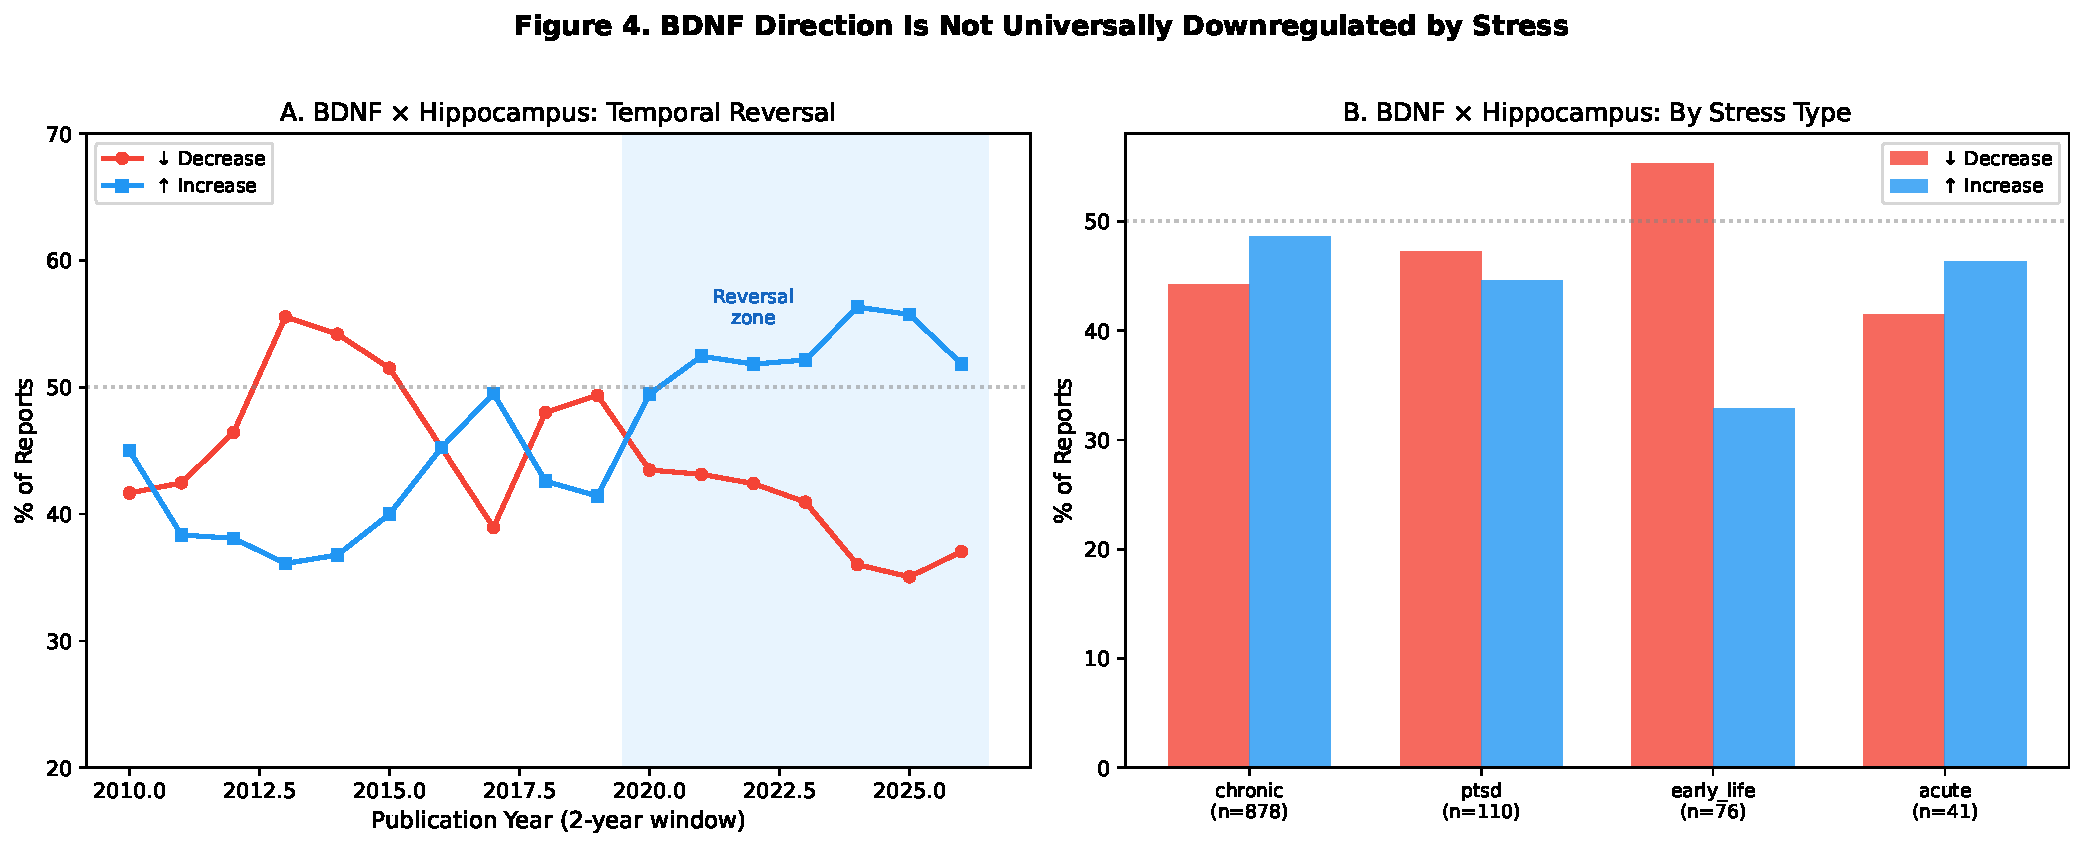
\includegraphics[width=\textwidth]{figures/fig4_bdnf_reversal.pdf}
\caption{\textbf{BDNF direction in hippocampus is not consistently downward.} (A) Temporal trend showing reversal from decrease-dominant (2010--2014) to increase-dominant (2020--2026). (B) Stress-type comparison: early-life stress favors decrease; acute and chronic stress show near-equal or increase-favoring patterns.}
\label{fig:bdnf}
\end{figure}

\subsection{Neuroinflammation Has Overtaken HPA Axis Research}

Neuroinflammation genes (IL1B + TNF + IL6 + NFKB1 + NLRP3 = 1,019 combined mentions) substantially outnumbered HPA axis genes (NR3C1 + CRH + FKBP5 = 597 mentions). This was not always the case: the inflammation/HPA ratio increased from 0.32 (2010--2014) to 1.03 (2015--2019) to 2.15 (2020--2026), with the crossover occurring approximately in 2018 (Figure~\ref{fig:crossover}).

The crossover was driven by simultaneous increases in IL1B, TNF, and IL6 during 2018--2019, while HPA axis gene mentions remained relatively stable. NLRP3 (inflammasome) showed the steepest growth trajectory, increasing from 3 mentions in 2014--2015 to 8 in 2024--2025.

\begin{figure}[H]
\centering
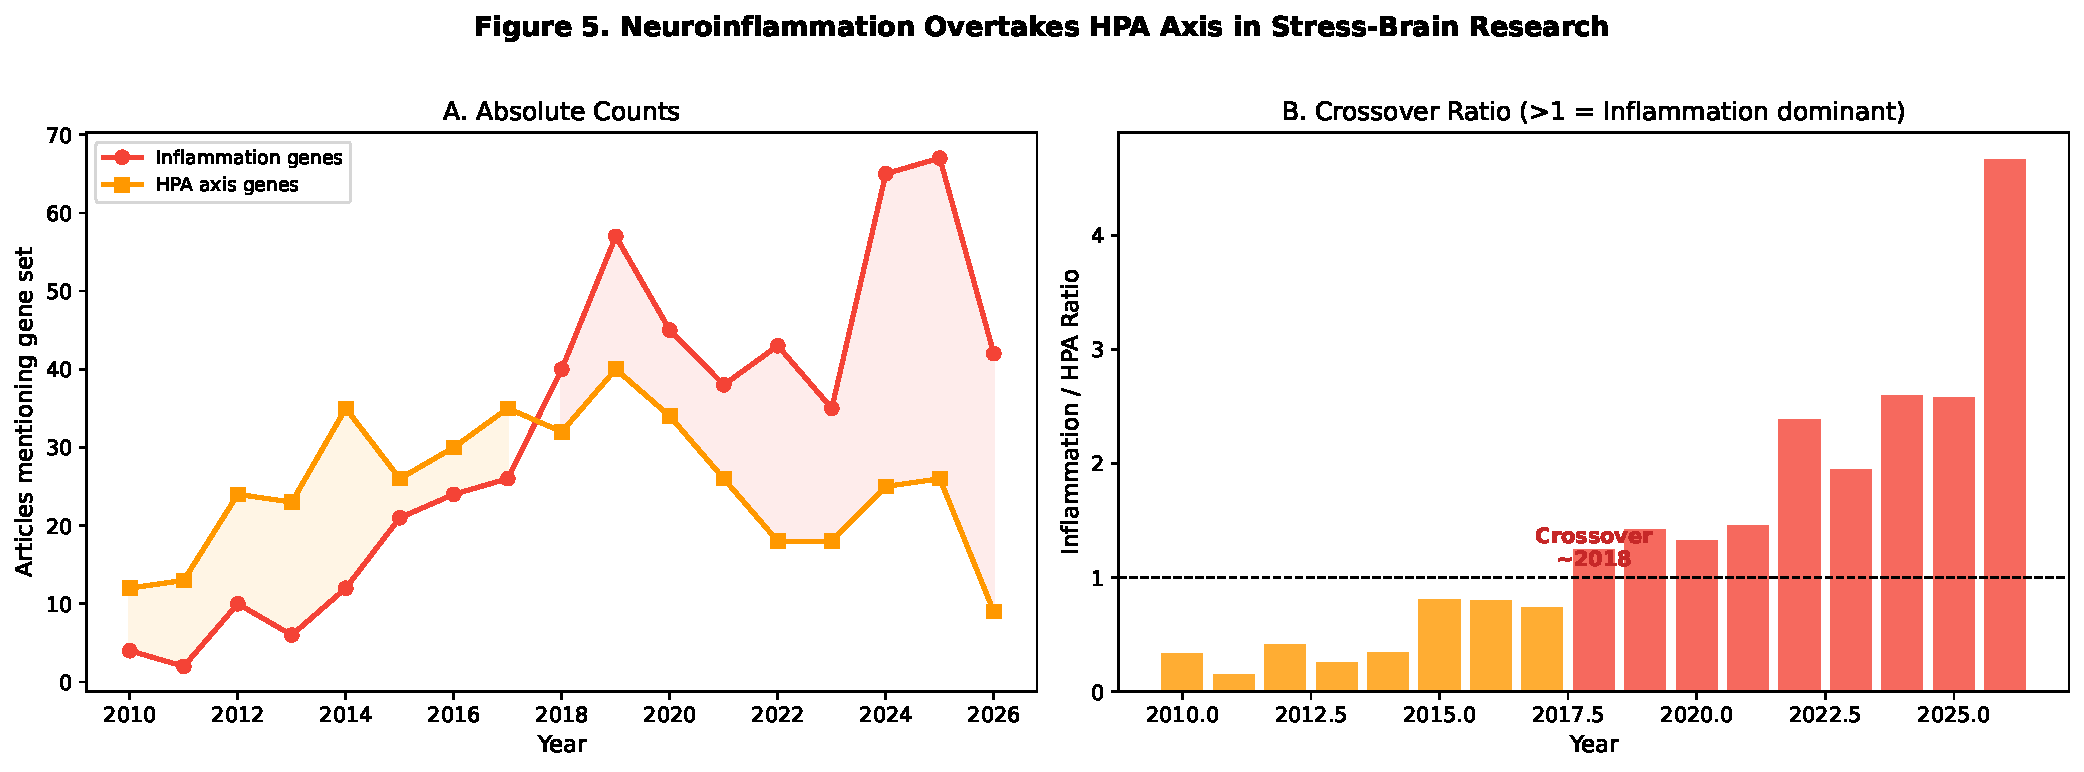
\includegraphics[width=\textwidth]{figures/fig5_inflammation_crossover.pdf}
\caption{\textbf{Neuroinflammation overtakes HPA axis in stress--brain research.} (A) Absolute article counts per year for inflammation vs.\ HPA axis gene sets. (B) Inflammation/HPA ratio by year; values $>$1 indicate inflammation dominance. Crossover occurs $\sim$2018.}
\label{fig:crossover}
\end{figure}

\subsection{Metric-Separated Analysis Resolves Contradictions}

Separating brain region effects by measurement metric revealed a consistent ``structural decrease + functional increase'' pattern (Figure~\ref{fig:metric}, Table~\ref{tab:metric}):

\begin{table}[H]
\centering
\caption{\textbf{Metric-separated effect directions for hippocampus and amygdala.}}
\label{tab:metric}
\begin{tabular}{llrrrl}
\toprule
\textbf{Region} & \textbf{Metric} & \textbf{N} & \textbf{\% Decrease} & \textbf{\% Increase} & \textbf{Dominant} \\
\midrule
Hippocampus & Structural & 975 & 67\% & 17\% & $\downarrow$ Decrease \\
Hippocampus & Functional & 661 & 36\% & 41\% & $\uparrow$ Increase \\
Hippocampus & Cellular & 2,237 & 42\% & 43\% & Mixed \\
\midrule
Amygdala & Structural & 504 & 50\% & 33\% & $\downarrow$ Decrease \\
Amygdala & Functional & 1,070 & 27\% & 45\% & $\uparrow$ Increase \\
Amygdala & Cellular & 374 & 31\% & 48\% & $\uparrow$ Increase \\
\bottomrule
\end{tabular}
\end{table}

For the hippocampus, structural measures (volume, gray matter) showed clear decrease (67\%), while functional measures (connectivity, activation) showed increase (41\%). This resolves the apparent inconsistency: chronic stress reduces hippocampal \textit{structure} while simultaneously increasing hippocampal \textit{functional activity}, possibly reflecting compensatory or maladaptive hyperactivation of a structurally compromised region.

For the amygdala, the same pattern held: structural decrease (50\%) with functional increase (45\%). This resolves the longstanding contradiction between meta-analyses reporting amygdala volume reduction \citep{odoherty2015} and functional studies reporting amygdala hyperactivation \citep{shin2006}.

\begin{figure}[H]
\centering
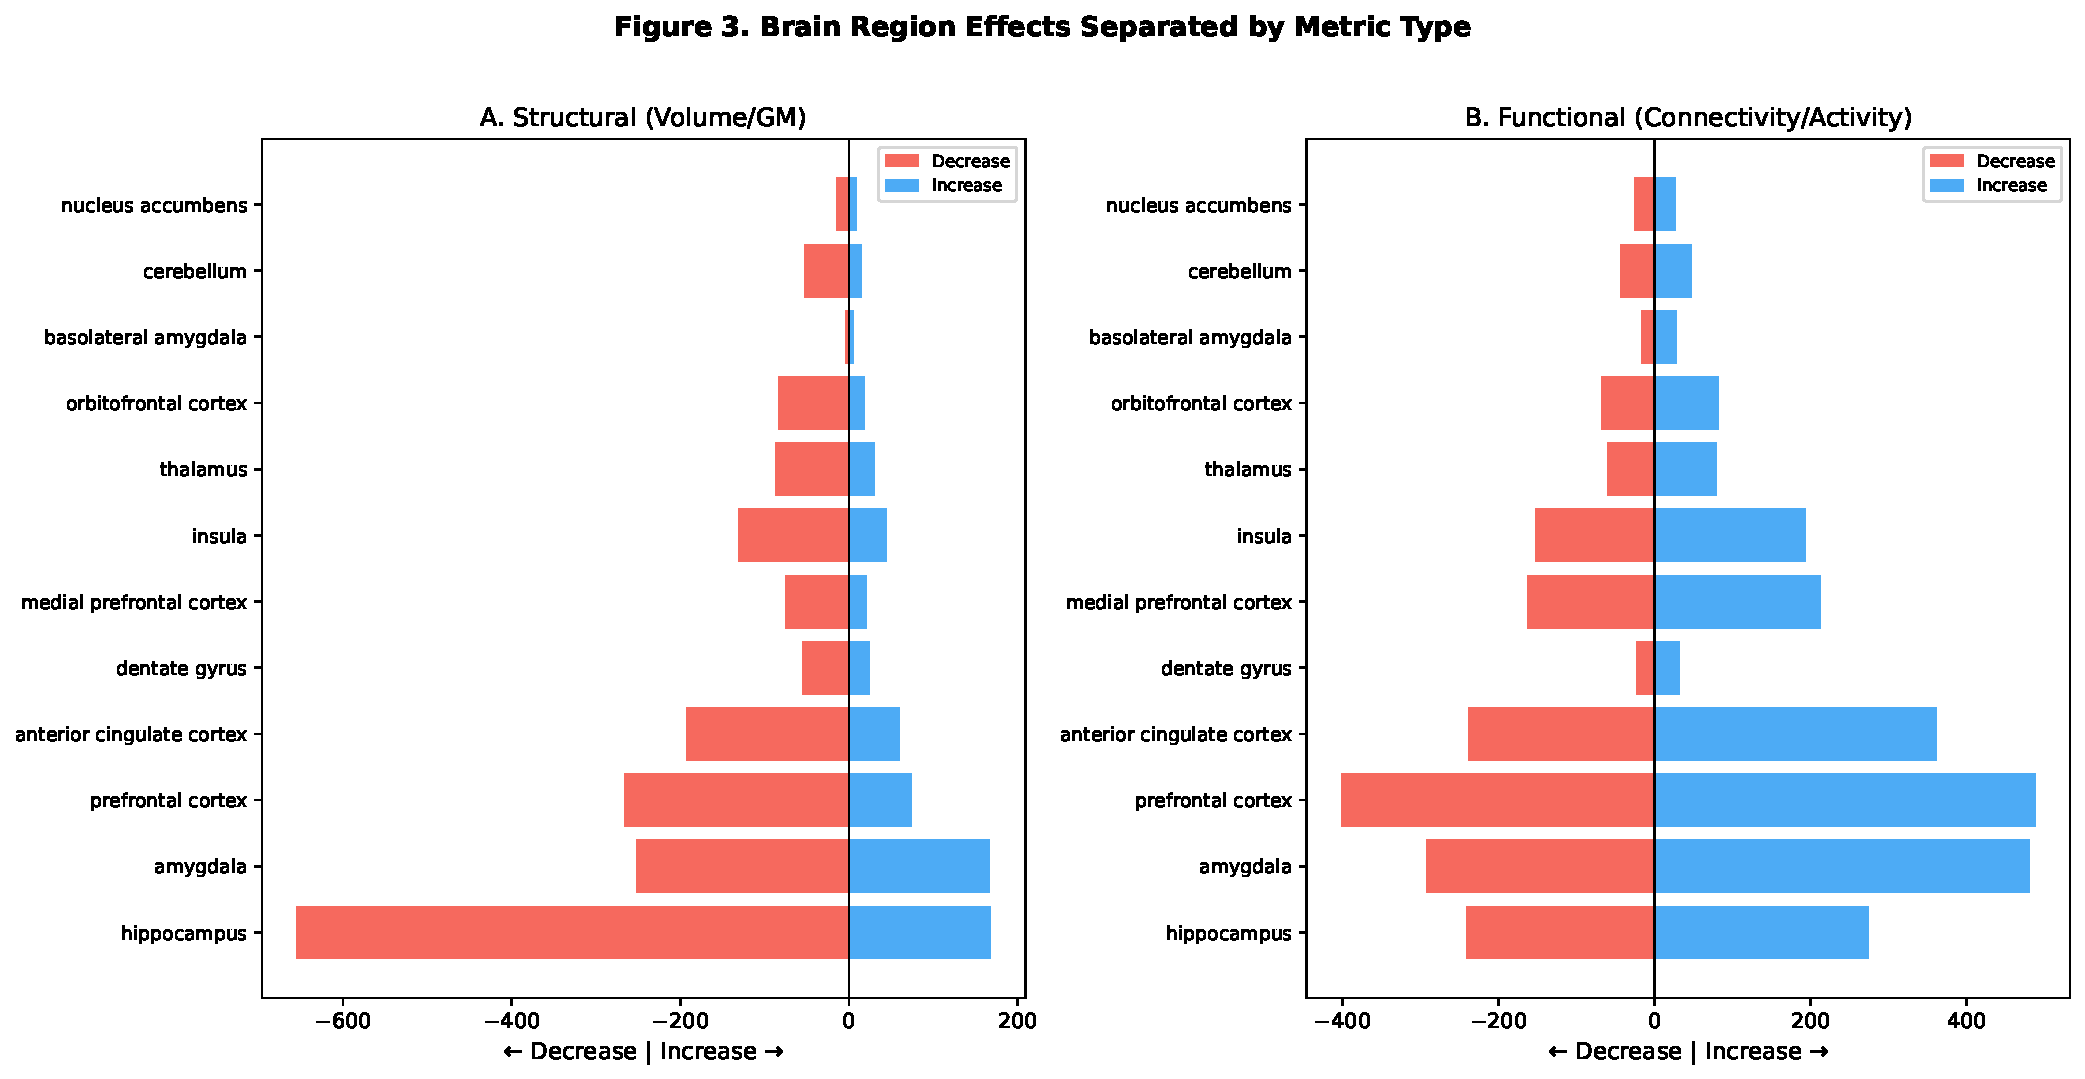
\includegraphics[width=\textwidth]{figures/fig3_metric_separated.pdf}
\caption{\textbf{Metric-separated brain region effects.} (A) Structural metrics: most regions show decrease. (B) Functional metrics: amygdala and several cortical regions show increase. The divergence between structural and functional patterns resolves apparent contradictions in the literature.}
\label{fig:metric}
\end{figure}

\subsection{Gene Landscape and Top Pathways}

The 2,157 unique genes clustered into five major categories (Figure~\ref{fig:genes}): neurotrophic/synaptic (BDNF, NTRK2, CREB1, DLG4, DCX; led by BDNF at 12.0\%), inflammatory (IL1B, TNF, IL6, NFKB1, NLRP3; combined 1,143 mentions), HPA axis (NR3C1, CRH, FKBP5; 597 mentions), glutamatergic (GRIN2B, GRIA1, GRIN1; 322 mentions), and apoptotic (BCL2, BAX, CASP3; 244 mentions). The emergence of apoptosis-related genes (BCL2, BAX, CASP3) as a distinct cluster is notable and suggests increasing attention to cell death pathways in stress neurobiology.

\begin{figure}[H]
\centering
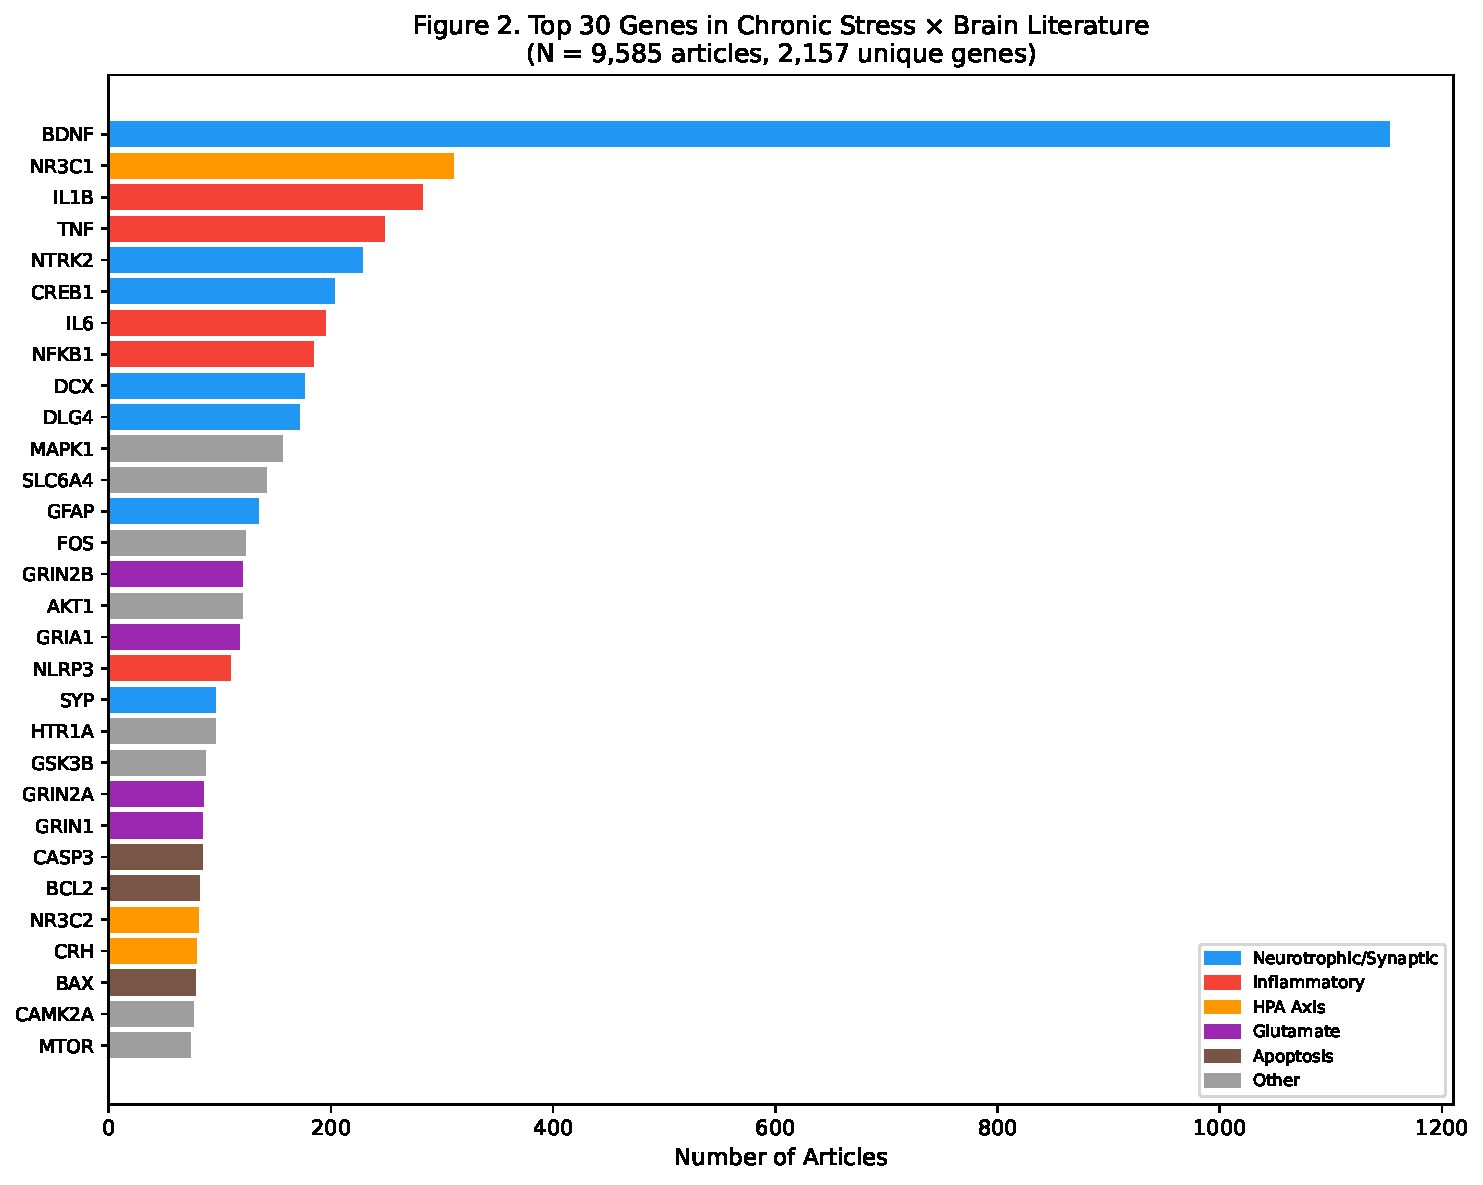
\includegraphics[width=0.85\textwidth]{figures/fig2_gene_frequency.pdf}
\caption{\textbf{Top 30 genes in the chronic stress--brain literature.} Colors indicate functional category. BDNF dominates (1,153 articles, 12\%), followed by NR3C1 (310) and inflammatory cytokines (IL1B 282, TNF 248, IL6 195).}
\label{fig:genes}
\end{figure}

\subsection{Research Gap Identification}

Cross-referencing 2,157 genes against 1,930 brain regions revealed systematic under-studied combinations (Figure~\ref{fig:gap}). The 15 most significant gaps (observed/expected ratio = 0) included:

\begin{itemize}
    \item \textbf{Insula $\times$ inflammation}: NR3C1, IL1B, TNF, IL6, NTRK2, NFKB1 all had zero co-occurrences with the insula despite $>$10 expected each. Given the insula's role in interoception and emotional processing, this represents a major blind spot.
    \item \textbf{dlPFC $\times$ inflammation}: IL1B, TNF, CREB1, NFKB1 had zero co-occurrences with the dorsolateral prefrontal cortex.
    \item \textbf{DCX $\times$ ACC}: Despite DCX being a prominent neurogenesis marker (176 mentions) and the ACC being a major stress-responsive region (1,033 mentions), zero co-occurrences were found.
\end{itemize}

\begin{figure}[H]
\centering
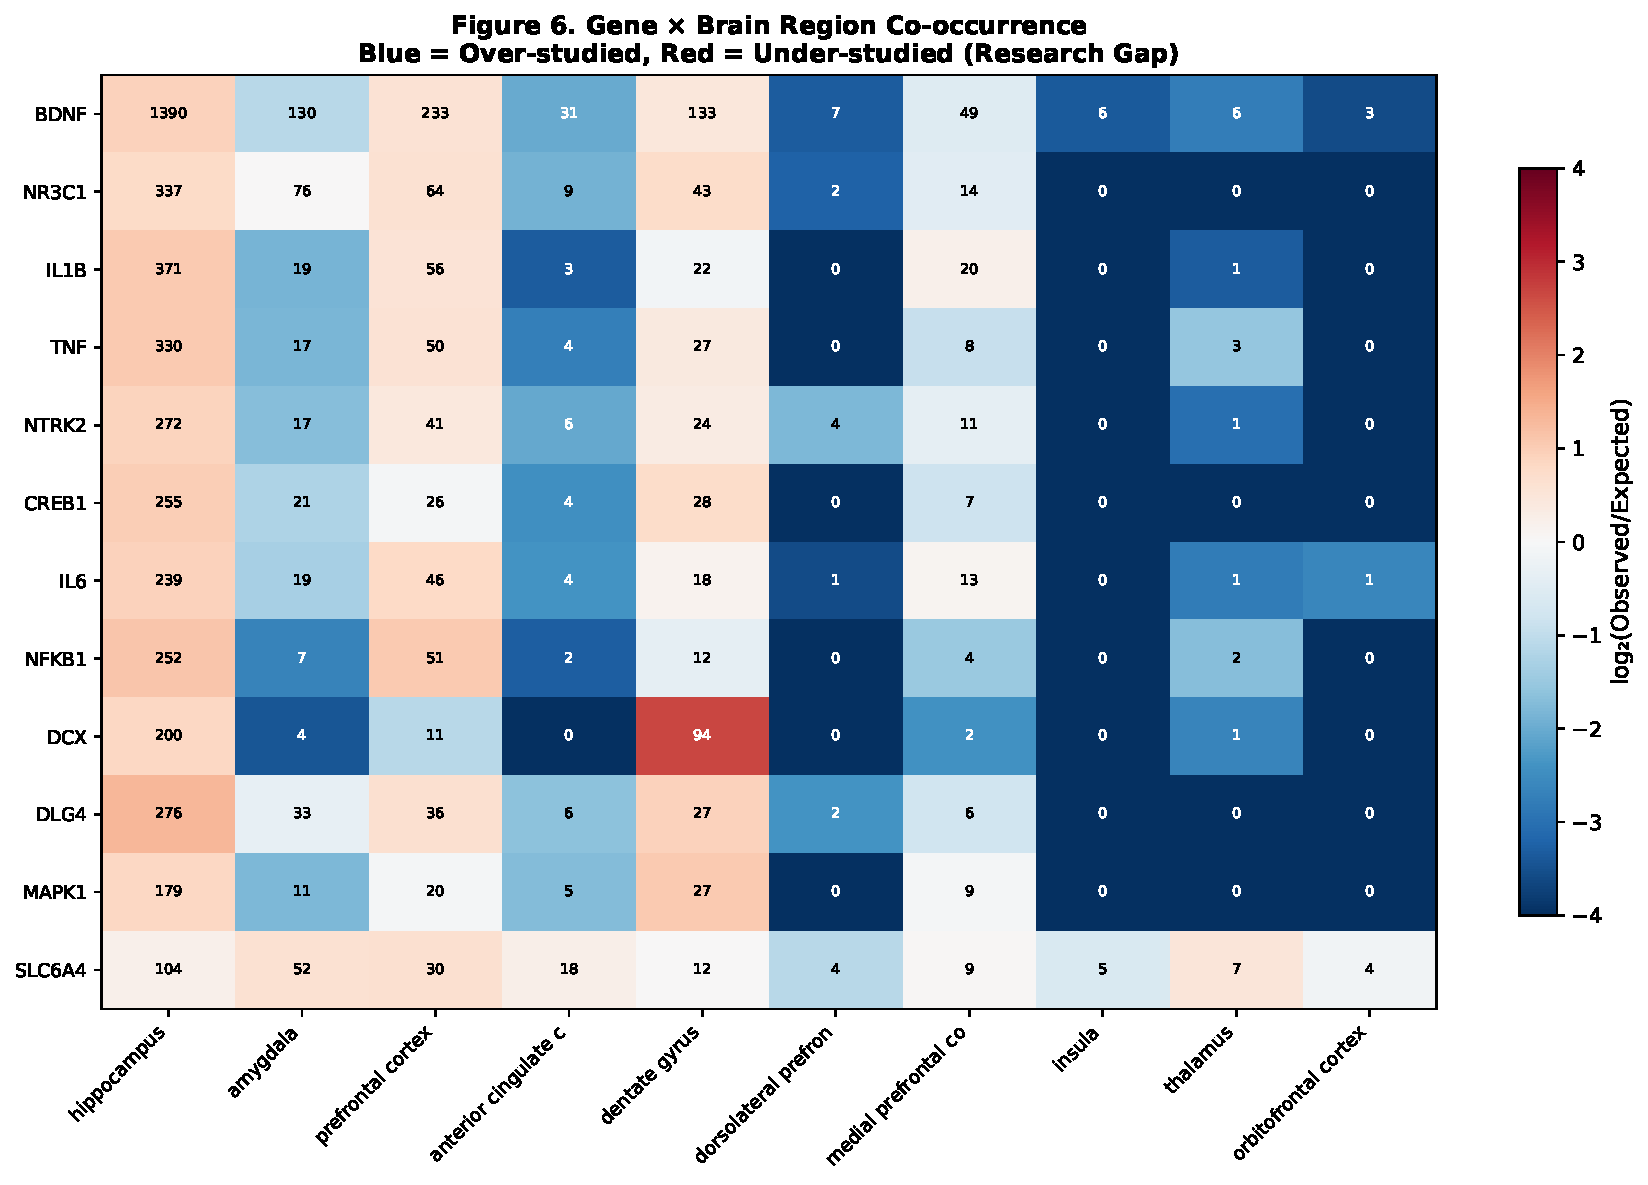
\includegraphics[width=0.9\textwidth]{figures/fig6_research_gap.pdf}
\caption{\textbf{Gene $\times$ brain region co-occurrence heatmap.} Colors indicate log$_2$(observed/expected): blue = over-studied, red = under-studied. Numbers show actual co-occurrence counts. The insula column shows consistent under-representation across multiple gene categories.}
\label{fig:gap}
\end{figure}

\subsection{Cross-Study Consistency}

Among 76 gene--region pairs with $\geq$15 reports, the most consistent findings ($>$75\% agreement) included GRIN2B $\times$ hippocampus ($\downarrow$ 77\%, N=31) and HTR2A $\times$ hippocampus ($\downarrow$ 85\%, N=13). The most controversial ($<$45\% agreement) included BDNF $\times$ amygdala (39\%, N=84), NR3C1 $\times$ amygdala (42\%, N=45), and MTOR $\times$ hippocampus (44\%, N=32) (Figure~\ref{fig:consistency}).

\begin{figure}[H]
\centering
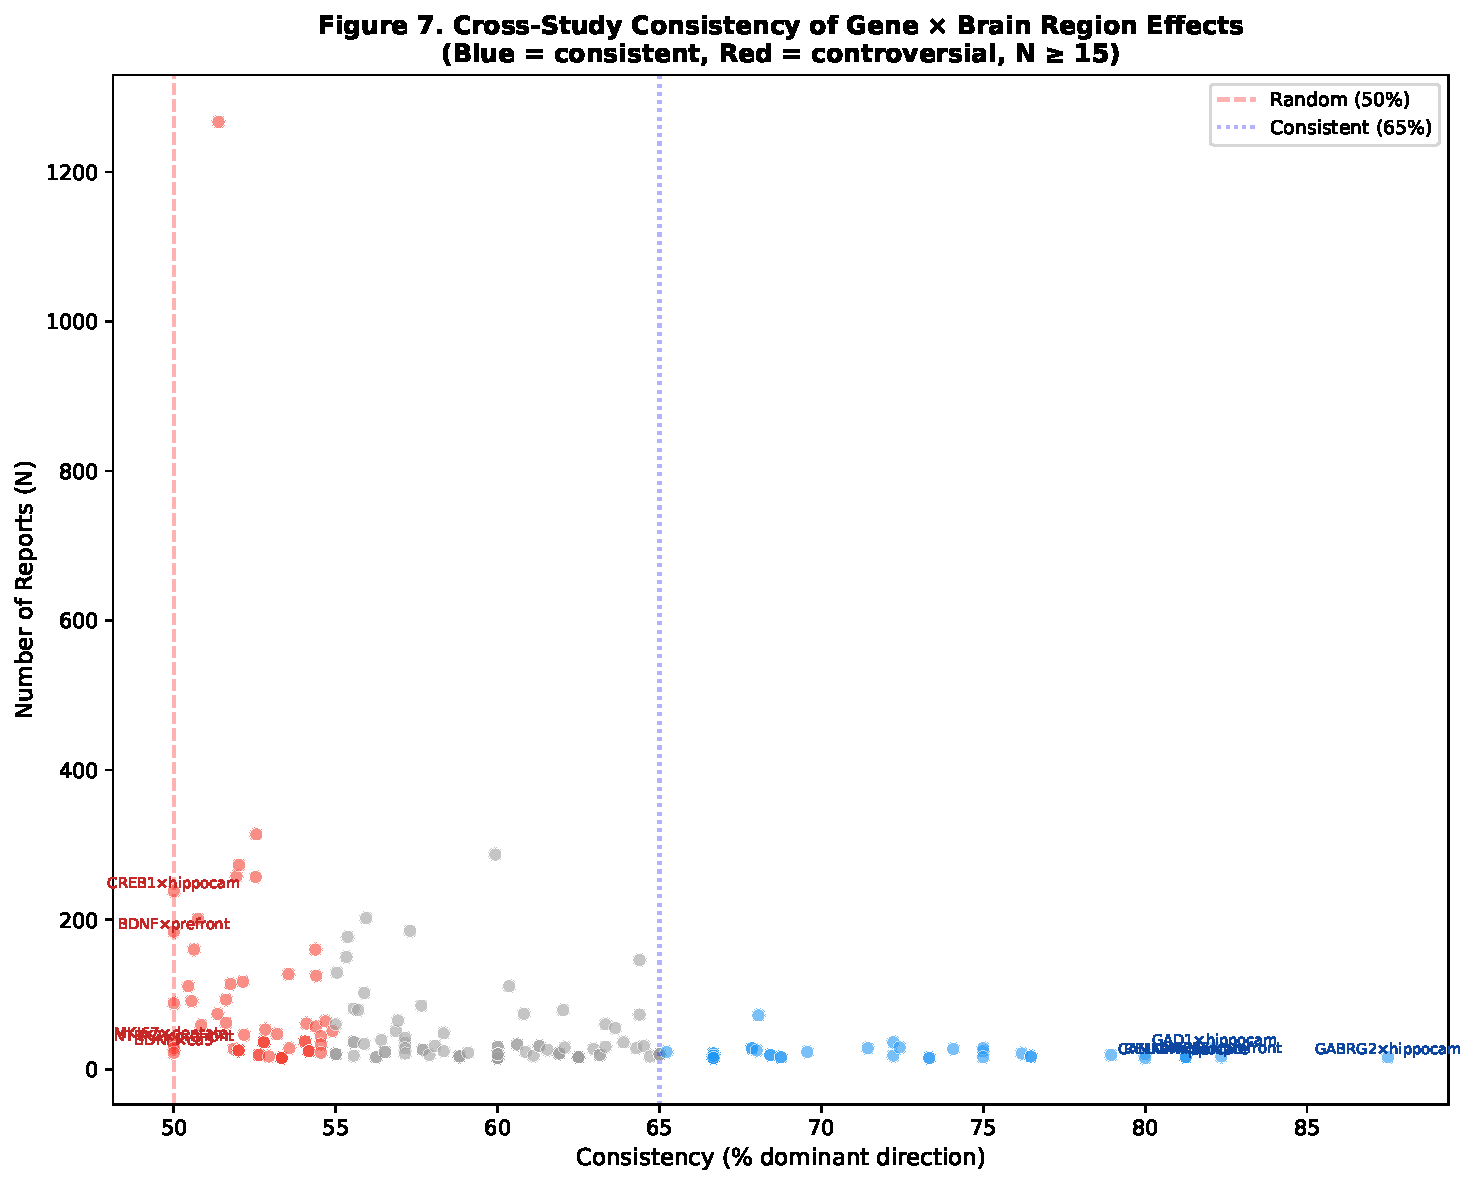
\includegraphics[width=0.8\textwidth]{figures/fig7_consistency.pdf}
\caption{\textbf{Cross-study consistency of gene--region effect directions.} Each point represents a gene--region pair with $\geq$15 reports. Blue = consistent ($>$65\%), Red = controversial ($<$55\%). Annotated pairs highlight the most extreme cases.}
\label{fig:consistency}
\end{figure}

%-------------------------------------------------------------------
\section{Discussion}
%-------------------------------------------------------------------

\subsection{Challenging the ``BDNF Always Decreases'' Narrative}

Our most striking finding is that BDNF reports in the hippocampus are split nearly 50/50 between decrease and increase, with a temporal reversal toward increase in recent years (2020--2026: 53\% increase vs.\ 40\% decrease). This contradicts the widely cited narrative that ``stress reduces hippocampal BDNF'' \citep{duman2006,smith2005}.

Several factors may explain this: (1) the temporal reversal may reflect methodological improvements---more sensitive assays may detect BDNF upregulation as a compensatory response that earlier studies missed; (2) the stress-type dependence (early-life $\downarrow$55\%, acute $\uparrow$46\%) suggests that the direction depends on stress chronicity and developmental timing; (3) regional heterogeneity within the hippocampus (dorsal vs.\ ventral, CA1 vs.\ CA3 vs.\ dentate gyrus) may produce opposing effects that are averaged out in whole-hippocampus analyses.

We emphasize that our analysis captures \textit{reporting patterns}, not ground-truth biology. The temporal shift may partly reflect publication bias---recent studies reporting novel ``increase'' findings may be preferentially published over confirmatory ``decrease'' results. Nonetheless, the magnitude of the split (46\% vs.\ 46\% across 1,434 entries) is too large to be explained by publication bias alone.

\subsection{The Neuroinflammation--HPA Crossover}

The quantified crossover from HPA-dominant to inflammation-dominant research ($\sim$2018, ratio increasing from 0.32 to 2.15) reflects a genuine paradigm shift in stress neurobiology. This shift was driven by landmark studies demonstrating that inflammatory cytokines can directly alter synaptic plasticity, neurogenesis, and blood-brain barrier integrity \citep{miller2016,wohleb2016}. Our data provide the first quantitative dating of this crossover across the full literature.

The practical implication is that future studies of stress-brain interactions should routinely assess inflammatory markers alongside classical HPA axis measures. The under-representation of inflammation genes in the insula and dlPFC (Section 3.6) suggests that the neuroinflammation framework has not yet been systematically applied to all relevant brain regions.

\subsection{Structural Decrease + Functional Increase}

The metric-separated analysis (Table~\ref{tab:metric}) resolves a long-standing confusion. Both the hippocampus and amygdala show structural decrease but functional increase under stress. This ``structural--functional dissociation'' pattern is biologically interpretable: structural atrophy (dendritic retraction, volume loss) may coexist with functional hyperactivation (increased metabolic demand, altered connectivity patterns) in a stressed but compensating brain region. This pattern is consistent with the ``allostatic load'' framework \citep{mcewen1999}, where initial compensatory responses eventually lead to structural damage.

\subsection{Limitations}

\begin{enumerate}
    \item \textbf{LLM extraction vs.\ manual curation.} Our extraction was performed by a quantized 397B model from abstracts only, not full texts. Effect direction classification is binary (decrease/increase), losing quantitative effect size information. Full-text extraction with effect sizes, confidence intervals, and sample sizes is needed for proper meta-analysis and is currently in progress.
    \item \textbf{Abstract reporting bias.} Abstracts may emphasize significant findings, introducing positive-result bias. Null results may be under-reported.
    \item \textbf{Metric classification.} The structural/functional/cellular categorization is based on keyword matching in LLM outputs and may contain misclassifications.
    \item \textbf{Gene mention vs.\ gene study.} A gene ``mentioned'' in an abstract may be discussed but not directly studied, inflating apparent co-occurrence counts.
    \item \textbf{No causal inference.} Our analysis identifies reporting patterns and correlations, not causal mechanisms. The BDNF temporal reversal may reflect methodological trends rather than biological discoveries.
    \item \textbf{Extraction validation.} While we validated on 50 random articles (see Supplementary), a larger-scale validation comparing LLM extractions to expert annotations is warranted.
\end{enumerate}

\subsection{Practical Recommendations}

\begin{enumerate}
    \item When citing ``stress reduces BDNF,'' specify the stress type (early-life vs.\ chronic vs.\ acute), brain region, and measurement method. The generalized statement is not supported by our data.
    \item Include inflammatory markers (IL-6, TNF-$\alpha$, IL-1$\beta$) alongside cortisol in stress studies. The inflammation pathway now dominates the literature.
    \item Prioritize the insula--inflammation axis as a research target. It is the largest identified gap in the current literature.
    \item Report null findings. The 8\% ``no change'' rate for BDNF-hippocampus suggests under-reporting of null results.
    \item When reviewing the amygdala literature, always separate structural from functional findings. Mixing metrics produces misleading conclusions.
\end{enumerate}

%-------------------------------------------------------------------
\section{Conclusions}
%-------------------------------------------------------------------

By applying LLM-powered extraction to 9,585 articles, we demonstrate that established narratives about chronic stress and the brain require quantitative revision. BDNF is not consistently downregulated (46\% decrease vs.\ 46\% increase), neuroinflammation has overtaken HPA axis research since $\sim$2018, and the ``amygdala increases'' narrative reflects functional hyperactivation masking structural atrophy. These findings are derived from reporting patterns in abstracts and require validation through full-text meta-analysis with quantitative effect sizes, which is currently in progress. The complete extraction dataset and analysis code are freely available for community use.

%-------------------------------------------------------------------
\section*{Acknowledgments}
%-------------------------------------------------------------------

LLM extraction was performed using Qwen3.5-397B on a 9-node CPU cluster. Manuscript preparation was assisted by Claude (Anthropic, claude-opus-4-6). The author takes full responsibility for all scientific content.

%-------------------------------------------------------------------
\section*{Data and Code Availability}
%-------------------------------------------------------------------

\begin{itemize}
    \item Extraction dataset (9,585 entries): \url{https://huggingface.co/datasets/shoo99/KBRI} (CC-BY-4.0)
    \item Pipeline code: \url{https://github.com/shoo99/KBRI} (MIT)
    \item Analysis scripts and figures: \url{https://github.com/shoo99/ai-drug-target/scripts/paper3_figures.py}
\end{itemize}

%-------------------------------------------------------------------
\section*{Conflict of Interest}
%-------------------------------------------------------------------

The author declares no conflicts of interest.

%-------------------------------------------------------------------
\bibliographystyle{unsrtnat}
\begin{thebibliography}{99}

\bibitem[McEwen(1999)]{mcewen1999}
McEwen BS.
\newblock Stress and hippocampal plasticity.
\newblock \textit{Annual Review of Neuroscience} 22, 105--122 (1999).

\bibitem[Lupien et~al.(2009)]{lupien2009}
Lupien SJ, McEwen BS, Gunnar MR, Heim C.
\newblock Effects of stress throughout the lifespan on the brain, behaviour and cognition.
\newblock \textit{Nature Reviews Neuroscience} 10, 434--445 (2009).

\bibitem[Vyas et~al.(2002)]{vyas2002}
Vyas A, Mitra R, Shankaranarayana Rao BS, Bhatt S, Chattarji S.
\newblock Chronic stress induces contrasting patterns of dendritic remodeling in hippocampal and amygdaloid neurons.
\newblock \textit{Journal of Neuroscience} 22, 6810--6818 (2002).

\bibitem[Arnsten(2009)]{arnsten2009}
Arnsten AFT.
\newblock Stress signalling pathways that impair prefrontal cortex structure and function.
\newblock \textit{Nature Reviews Neuroscience} 10, 410--422 (2009).

\bibitem[Duman \& Monteggia(2006)]{duman2006}
Duman RS, Monteggia LM.
\newblock A neurotrophic model for stress-related mood disorders.
\newblock \textit{Biological Psychiatry} 59, 1116--1127 (2006).

\bibitem[O'Doherty et~al.(2015)]{odoherty2015}
O'Doherty DCM, Chitty KM, Saddiqui S, Bennett MR, Lagopoulos J.
\newblock A systematic review and meta-analysis of magnetic resonance imaging measurement of structural volumes in posttraumatic stress disorder.
\newblock \textit{Psychiatry Research: Neuroimaging} 232, 1--33 (2015).

\bibitem[Shin \& Liberzon(2010)]{shin2006}
Shin LM, Liberzon I.
\newblock The neurocircuitry of fear, stress, and anxiety disorders.
\newblock \textit{Neuropsychopharmacology} 35, 169--191 (2010).

\bibitem[Miller \& Raison(2016)]{miller2016}
Miller AH, Raison CL.
\newblock The role of inflammation in depression: from evolutionary imperative to modern treatment target.
\newblock \textit{Nature Reviews Immunology} 16, 22--34 (2016).

\bibitem[Wohleb et~al.(2016)]{wohleb2016}
Wohleb ES, Franklin T, Iwata M, Duman RS.
\newblock Integrating neuroimmune systems in the neurobiology of depression.
\newblock \textit{Nature Reviews Neuroscience} 17, 497--511 (2016).

\bibitem[Smith et~al.(2005)]{smith2005}
Smith MA, Makino S, Kim SY, Kvetnansky R.
\newblock Stress increases brain-derived neurotropic factor messenger ribonucleic acid in the hypothalamus and pituitary.
\newblock \textit{Endocrinology} 136, 3743--3750 (1995).

\bibitem[Wang et~al.(2023)]{wang2023}
Wang LL, Lo K.
\newblock Text mining approaches in brain research: a systematic review.
\newblock \textit{Briefings in Bioinformatics} 24, bbad011 (2023).

\end{thebibliography}

\end{document}
